\documentclass{beamer}
\usepackage{graphicx}
\usepackage{amsmath}
\usepackage{booktabs}
\usepackage[utf8]{inputenc}
\usepackage[T1]{fontenc}

\title{Coupling SciMBA and Feel++}
\author{Abdoul Aziz Sarr \and Yehua He}
\date{April 2025}

\begin{document}

\maketitle

% Section: Context
\section{Context}
\begin{frame}{Context}
  The project is part of \textbf{Exa-MA}, aiming to develop \textbf{exascale numerical methods} and \textbf{open-source libraries} for next-generation supercomputers.

  The goal is to couple traditional simulations (finite elements) with AI techniques through the integration of:
  \begin{itemize}
    \item \textbf{Feel++}: finite element PDE solver
    \item \textbf{SciMBA}: scientific machine learning framework
  \end{itemize}
\end{frame}

% Motivation Slide
\begin{frame}{Motivation: Hybridizing FEM with Neural Networks}
We explore a hybrid strategy that combines:
\begin{itemize}
  \item \textbf{Classical FEM}: accurate, with known error estimators
  \item \textbf{Neural networks (PINNs)}: fast, flexible, but less precise
\end{itemize}

\vspace{1em}
\textbf{Idea:} enrich the continuous Lagrange finite element space by incorporating prior knowledge from neural network predictions.

\begin{itemize}
  \item Improves initial approximation and reduces degrees of freedom
  \item Error estimates depend on prior quality
  \item Allows use of \textbf{coarser meshes} to reach a target error faster
\end{itemize}
\end{frame}

% Section: Libraries
\section{Libraries}

\begin{frame}{Library: Feel++}
  \begin{itemize}
    \item C++/Python library for PDE solving using the \textbf{Galerkin method}
    \item Generates finite element solutions on structured/unstructured meshes
    \item Operates on \textit{\(P_k^c\) Lagrange finite element spaces}
  \end{itemize}
\end{frame}

\begin{frame}{Library: SciMBA}
  \begin{itemize}
    \item Python library for scientific machine learning
    \item Implements \textbf{PINNs} and \textbf{neural operators}
    \item Outputs can be used as boundary/initial conditions or surrogate solutions
  \end{itemize}
\end{frame}

% Section: Coupling
\section{Coupling Strategy}
\begin{frame}{Coupling SciMBA–Feel++}
  \textbf{Core mechanism:} memory interface via \textbf{PyBind11}
  \begin{enumerate}
    \item Direct in-memory data exchange (e.g. vectors/tensors)
    \item Construction of \( P_k^c \) Lagrange interpolants:
    \[
      u_h(\xi_i) = \hat{u}_\theta(\xi_i)
    \]
    \item Reuse in Feel++ simulations (source terms, boundary values)
  \end{enumerate}
\end{frame}

% Section: Projects
\section{Projects}

\begin{frame}{Project 1: PINNs vs FEM Benchmark (Poisson)}
  \textbf{Goal:} Compare PINN (SciMBA) and FEM (Feel++) solutions
  \begin{itemize}
    \item PINN formulation:
    \[
      \hat{u}_\theta = \arg\min \frac{1}{M} \sum (-\Delta u(x_i) - f(x_i))^2
    \]
    \item FEM: Solve weak formulation \( a(u, v) = l(v) \)
    \item Metrics: $L^2$ and $H^1$ error, visual comparisons, interpolation quality
  \end{itemize}
\end{frame}

\begin{frame}{Project 2: Neural Operator Surrogate}
  \textbf{Parametric diffusion equation}
  \begin{itemize}
    \item Train Fourier operator on Feel++-generated FEM solutions
    \item Learn mapping \( \mu \mapsto u(x,y;\mu) \)
    \item Predict new solutions and inject via interpolants
  \end{itemize}
\end{frame}

\begin{frame}{Project 3: Hybrid FEM–PINN Domain Decomposition}
  \begin{itemize}
    \item Split domain, e.g., \([0, 0.5]\) FEM, \([0.5, 1]\) PINN
    \item Neumann interface at midpoint
    \item Exchange data at boundary via memory coupling
    \item Challenge: smoothness, consistency, convergence
  \end{itemize}
\end{frame}

% Numerical Validation Slide
\begin{frame}{Numerical Validation (Preliminary)}
\begin{itemize}
  \item Validated on 1D and 2D parametric PDEs
  \item Enhanced FEM with neural priors achieves same error as standard FEM with \textbf{fewer elements}
  \item Leads to faster computations for parametric sweeps
  \item Highlights benefit of blending fast neural approximations with certified FEM accuracy
\end{itemize}

\vspace{0.5em}
\textit{This supports further development of hybrid PDE solvers.}
\end{frame}

% Implementation Focus
\section{Implementation Focus}

\begin{frame}{Technical Comparison}
\resizebox{\textwidth}{!}{ 
\begin{tabular}{lll}
\toprule
\textbf{Aspect} & \textbf{PINNs} & \textbf{FEM} \\
\midrule
Formulation & Strong residual minimization & Variational (weak) formulation \\
Computational cost & High (training required) & Deterministic linear/nonlinear solve \\
Flexibility & Adaptive to parameter change & Precise for known problems \\
\bottomrule
\end{tabular}}
\end{frame}

\begin{frame}{Expected Results and Deliverables}
\begin{itemize}
  \item Functional SciMBA–Feel++ interface for PINN prediction injection
  \item PINN solution quality benchmarked against FEM
  \item Error metrics ($L^2$ and $H^1$ norms), interpolation accuracy
  \item Final deliverables:
  \begin{itemize}
    \item C++/Python codebase
    \item Interpolation module
    \item Final report + presentation
  \end{itemize}
\end{itemize}
\end{frame}

\begin{frame}{Example: Visualizing the solution for a Laplacian problem}
\begin{figure}
    \centering
    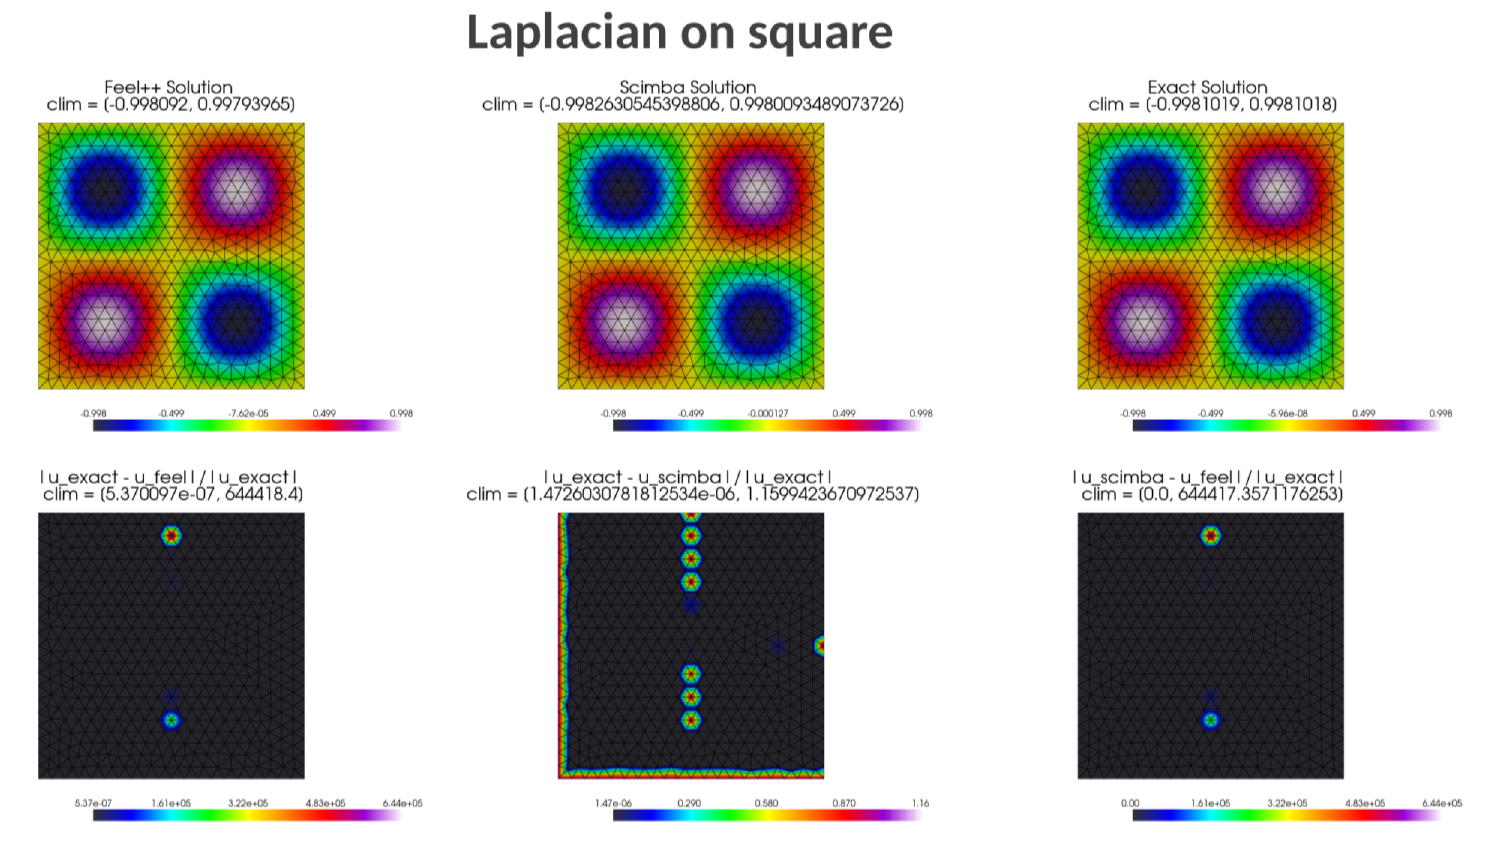
\includegraphics[width=1\linewidth]{docs//proposals//2025//images/laplacian.png}
    \label{fig:enter-label}
\end{figure}
\end{frame}

% Conclusion
\begin{frame}{Conclusion}
\begin{itemize}
  \item This project bridges traditional numerical methods and scientific ML.
  \item Direct coupling enables hybrid PDE solvers leveraging both PINNs and FEM.
  \item This coupling framework lays the foundation for scalable solvers in high-dimensional, multi-physics problems.
\end{itemize}
\vspace{1em}
\centering
\textbf{Thank you for your attention!} \\
\texttt{yehua.he@etu.unistra.fr} \quad \texttt{abdoul.sarr@etu.unistra.fr}
\end{frame}



\end{document}
